\documentclass{beamer}
\usetheme{Berkeley}
\usecolortheme{wolverine}
\usepackage{graphicx}
\usepackage[utf8]{inputenc}

\title{Merge Sort and Counting Sort}
\subtitle{C.S.E.-2200}
\author[Md. Shahidul Islam Dipu \and Zabed Iqbal]{SLide Creation \newline\and Md. Shahidul Islam Dipu (2003040) \newline\and Zabed Iqbal (2003011)
	\newline Article Writting :\newline MD. Sartaj Alam Pritom 
	(2003046) 
	\newline\and Nafis Raihan (2003005)
	\newline\and Latex Creation : 
	\newline\and Raihan UL Islam (2003006)
	\newline\and Soscho Shamuel Gregory (2003007)

}


\begin{document}
	
	\begin{frame}
		\titlepage
	\end{frame}
	
	\begin{frame}{Outline}
		\tableofcontents
	\end{frame}
	
	\section{Abstract}
	
	\begin{frame}{Abstract}
		\begin{itemize}
			\item \textbf{Objective:} Conduct a comparative analysis of Merge Sort and Counting Sort.
			
			\item \textbf{Focus:} Evaluate performance across diverse dataset sizes.
			
			\item \textbf{Complexities:} Explore time (Merge Sort: $O(n \log n)$, Counting Sort: $O(n + k)$) and space complexities.
			
			\item \textbf{Characteristics:} Merge Sort's versatility suits various datasets; Counting Sort excels in linear efficiency, ideal for large datasets with limited value ranges.
			
			\item \textbf{Methodology:} Systematic experimentation with varying dataset sizes.\cite{researchgate}
		\end{itemize}
	\end{frame}
	
	\begin{frame}{Abstract}
		\begin{itemize}
			\item \textbf{Findings:} Empirical evidence on sorting algorithms' performance.
			
			\item \textbf{Implications:} Practical insights for real-world algorithm selection.
			
			\item \textbf{Limitations:} Acknowledge dataset-related constraints.
			
			\item \textbf{Recommendations:} Optimize Merge Sort; explore additional sorting algorithms.
			
			\item \textbf{Conclusion:} Concise analysis aids sorting algorithm discussions for researchers and practitioners.
		\end{itemize}
	\end{frame}
	
	\section{Introduction}
	
	\begin{frame}{Introduction}
		\begin{itemize}
			\item Sorting algorithms significantly impact computer science applications.
	
			\item Efficient data organization and retrieval are crucial in modern computing.
			
			\item Sorting algorithms play a pivotal role in diverse applications. \cite{cormen2009introduction}
		\end{itemize}
	\end{frame}
	
	\begin{frame}{Introducing Merge Sort and Counting Sort}
		\begin{itemize}
			\item \textbf{Merge Sort:} Known for elegance and reliability. Efficiently breaks down and merges datasets, ensuring intricately ordered data.
			
			\item \textbf{Counting Sort:} A non-comparative algorithm with $O(n + k)$ complexity. Particularly effective in sorting integers and character frequencies within limited value range datasets.
		\end{itemize}
	\end{frame}
	
	\begin{frame}{Introducing Merge Sort and Counting Sort (cont.)}
		\begin{itemize}
			
			\item \textbf{Applications:}
			
			\textit{Merge Sort:} Ideal for stable sorting in data processing and scientific computing.
			
			\textit{Counting Sort:} Efficient for sorting integers and character frequencies.
			
			\item Both algorithms contribute to real-world scenarios.
		\end{itemize}
	\end{frame}
	
	\begin{frame}{Objectives of this Study}
		\begin{itemize}
			\item This research aims to compare Merge Sort and Counting Sort comprehensively.
			
			\item Evaluate theoretical foundations and practical performance on diverse datasets.
			
			\item Provide nuanced insights into trade-offs and advantages of each algorithm. \cite{googlescholar}
		\end{itemize}
	\end{frame}
\section{Background Study}

\subsection{Merge Sort}

\begin{frame}{Background Study: Merge Sort Overview}
	\begin{itemize}
		\item \textbf{Divide and Conquer:} Merge Sort employs a "divide and conquer" strategy, breaking down the sorting process into smaller, more manageable tasks.
		\item \textbf{Recursive Sorting:} It recursively divides the array into halves until individual elements, then merges them in a sorted manner.
		\item \textbf{Time Complexity:} Exhibits a time complexity for both Average and Worst case of $O(n \log n)$, making it efficient for large datasets.
		\item \textbf{Space Complexity:} Requires $O(n)$ auxiliary space for the merging operation. \cite{geeksforgeeks-merge-sort}
	\end{itemize}
\end{frame}

\begin{frame}[fragile]{Background Study: Merge Sort Algorithm (Merge)}
	\begin{verbatim}
		merge(left, right):
		result = []
		left_index = right_index = 0
		
		while left_index < length(left) 
		and right_index < length(right):
		if left[left_index] < right[right_index]:
		result.append(left[left_index])
		left_index++
		else:
		result.append(right[right_index])
		right_index++
		
		result.extend(left[left_index:])
		result.extend(right[right_index:])
		
		return result
	\end{verbatim}
\end{frame}

\begin{frame}[fragile]{Background Study: Merge Sort Algorithm (MergeSort)}
	\begin{verbatim}
		mergeSort(arr):
		if length(arr) <= 1:
		return arr
		
		mid = length(arr) / 2
		left_half = mergeSort(arr[0:mid])
		right_half = mergeSort(arr[mid:])
		return merge(left_half, right_half)
	\end{verbatim}
	Merge Sort recursively dissects datasets, sorting smaller components, and seamlessly merges them back into wholes. This divide-and-conquer strategy ensures ordered data and optimization for efficient retrieval.
\end{frame}

\begin{frame}{Background Study: Merge Sort Visualization}
	\begin{figure}
		\centering
		%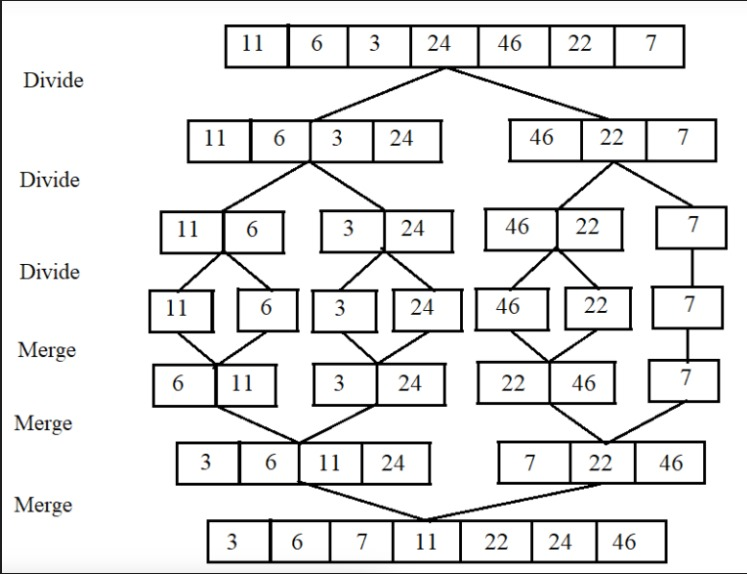
\includegraphics[width=0.7\linewidth]{WhatsApp Image 2024-01-21 at 20.15.55_26ce695b.jpg}
		\caption{Process of MergeSort}
		\label{fig:enter-label}
	\end{figure}
\end{frame}

\subsection{Counting Sort}

\begin{frame}{Background Study: Counting Sort Overview}
	\begin{itemize}
		\item \textbf{Counting Sort Overview:} Counts the occurrences of each element in the input. Calculates the cumulative count of elements. Places elements in their correct, sorted positions.
		\item \textbf{Time Complexity:} Demonstrates a time complexity of $O(n + k)$, where $k$ is the range of input. Exhibits stability, maintaining the order of equal elements.
		\item \textbf{Space Complexity:} Requires $O(k)$ additional space for the counting array.
		\item \textbf{Visualization:} Visual representation aids in understanding the counting and placement process.
	\end{itemize}
\end{frame}

\begin{frame}[fragile]{Background Study: Counting Sort Algorithm}
	\begin{verbatim}
		Count array C[0..k] initialized to 0;
		for i from 1 to n do
		C[A[i]] += 1;
		for i from 1 to k do
		C[i] += C[i-1];
		for i from n to 1 do
		B[C[A[i]]] = A[i];
		C[A[i]] -= 1;
	\end{verbatim}
	Counting Sort begins by creating an array filled with zeros and counting occurrences of each distinct element. It then calculates positions for elements and efficiently places them in their final order.\cite{geeksforgeeks-counting-sort}
\end{frame}

	
\section{Results and Analysis}
\subsection{Introduction to Results}
\begin{frame}{Result and Analysis}
	\begin{itemize}
		
		\item \textbf{Introduction to Results:}
		\begin{itemize}
			\item This experiment meticulously evaluates and compares Merge Sort and Counting Sort, two fundamental sorting algorithms.
			\item Sorting algorithms are crucial in computer science and data processing, impacting the efficiency and speed of applications.
			\item Our study aims to analyze algorithm performance across a spectrum of dataset sizes, from small to significantly large datasets. \cite{Wikipedia}
		\end{itemize}
		
		\item \textbf{Dataset Variation and Configuration:}
		\begin{itemize}
			\item Datasets of varying sizes (10,000 to 100,000 data points) were configured for a comprehensive algorithm performance assessment.
			\item The selected datasets represent practical scenarios, covering everyday modest-sized datasets to extensive datasets reflecting substantial data processing demands.
		\end{itemize}
	\end{itemize}
	
\end{frame}

\subsection{Execution Times}

\begin{frame}{Execution Time}
	\begin{table}
		\centering
		\begin{tabular}{|c | c | c|} 
			\hline
			Data Size  & Merge Sort Time(ms)  & Counting Sort Time(ms) \\ [0.5ex]
			\hline
			10000 & 4074.8 & 534.5 \\
			\hline
			20000 & 8387.2 & 691.9 \\
			\hline
			30000 & 13791.6 & 979.9 \\
			\hline
			40000 & 17537.1 & 1141.7 \\
			\hline
			50000 & 22100.3 & 1336.2 \\
			\hline
			60000 & 26453.6 & 1571 \\
			\hline
			70000 & 31218.4 & 1709.2 \\
			\hline
			80000 & 35476 & 1955.8 \\
			\hline
			90000 & 40404.9 & 2691.7 \\
			\hline
			100000 & 45341.8 & 3288.1 \\
			\hline
		\end{tabular}
		\caption{Execution times for Merge Sort and Counting Sort}
	\end{table}
\end{frame}

\subsection{Graph}
\begin{frame}{Graph}
	\begin{figure}
		\centering
		%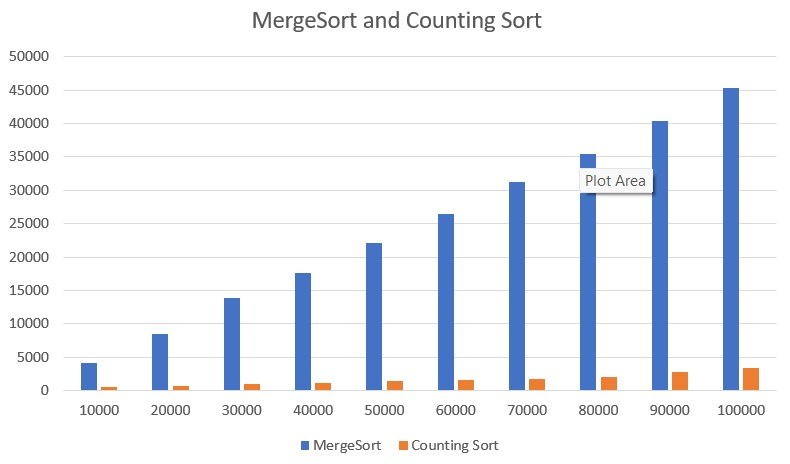
\includegraphics[width=1\linewidth]{BAR}
		\caption{Performance analysis comparison}

	\end{figure}
	
\end{frame}

		
\subsection{Analysis}

\begin{frame}{Observations}
	\begin{itemize}
		\item \textbf{Merge Sort:}
		\begin{itemize}
			\item Time increases consistently with the growth of the dataset.
			\item Reflects the expected behavior of \(O(n \log n)\) time complexity.
			\item Non-linear increase indicates the influence of the logarithmic factor.
		\end{itemize}
		\item \textbf{Counting Sort:}
		\begin{itemize}
			\item Demonstrates consistently lower times compared to Merge Sort.
			\item Linear time complexity (\(O(n + k)\)) contributes to its efficiency, especially for smaller datasets.
		\end{itemize}
	\end{itemize}
\end{frame}

\begin{frame}{Explanation}
	\begin{itemize}
		\item \textbf{Merge Sort:}
		\begin{itemize}
			\item Performs well but exhibits a logarithmic growth in time.
			\item Becomes relatively more efficient as dataset size increases.
		\end{itemize}
		\item \textbf{Counting Sort:}
		\begin{itemize}
			\item Maintains efficiency across all dataset sizes.
			\item Linear time complexity allows for faster sorting, especially for smaller datasets.
		\end{itemize}
	\end{itemize}
\end{frame}

\begin{frame}{Recommendations}
	\begin{itemize}
		\item \textbf{For Smaller Datasets:}
		\begin{itemize}
			\item \textit{Counting Sort:} Highly efficient due to its linear time complexity. Recommended for datasets with limited sizes.
		\end{itemize}
		\item \textbf{For Larger Datasets:}
		\begin{itemize}
			\item \textit{Merge Sort:} Becomes a competitive and efficient choice as dataset size increases. Balances efficiency and stability for larger and more complex datasets.
		\end{itemize}
	\end{itemize}
\end{frame}

\begin{frame}{Practical Implications and Recommendations}
		\begin{itemize}
			\item \textbf{Merge Sort:}
			\begin{itemize}
				\item Suitable for general-purpose sorting where stability and adaptability are crucial.
				\item Versatile, making it viable for diverse sorting requirements in manageable dataset sizes.
				\item Particularly beneficial when a stable sorting algorithm is required.
			\end{itemize}
			
			\item \textbf{Counting Sort:}
			\begin{itemize}
				\item Ideal for scenarios with a limited range of values.
				\item Efficient and scalable, particularly advantageous for large datasets.
				\item Well-suited for situations with a constrained range, prioritizing sorting speed over versatility.
			\end{itemize}
		\end{itemize}

\end{frame}


	\section{Conclusion}
	
	\begin{frame}{Conclusion}
		\begin{itemize}
			\item The comprehensive comparison between Merge Sort and Counting Sort has illuminated their distinct characteristics.
			\item Merge Sort, though stable, demonstrated limitations in efficiency for larger or complex datasets, aligning with its expected time complexity growth of \(O(n \log n)\).
			\item Counting Sort's linear time complexity (\(O(n + k)\)) showcased remarkable efficiency, particularly excelling in scenarios with large datasets.
		\end{itemize}
		
		
		\begin{itemize}
			\item The findings endorse Counting Sort as a preferred choice for fast sorting in applications prioritizing sorting speed.
			\item Its adaptability to diverse real-world scenarios offers valuable insights for algorithm selection.
			\item The study underscores the significance of considering algorithmic characteristics and real-world requirements when choosing sorting methods, ultimately guiding towards informed and effective decision-making.
		\end{itemize}
	\end{frame}
	
	\section{Reference}
	\begin{frame}
		\frametitle{Reference}
		\bibliographystyle{acm}
	\bibliography{refs}
	\end{frame}
	
	
	
	\begin{frame}
		\begin{center}
			\textbf{THANK YOU}
		\end{center}    
	\end{frame}
	
\end{document}